%!TEX root = ../Thesis.tex

\section{Planar Assumption and Intersection Least squares results}
These results had no error induced in the measurements in order to analyse the effectiveness and robustness of the algorithm. No epoch alignment and no correlated or uncorrelated errors. Only two receivers were used with the reference receiver exactly at the approximate location. The second receiver was set at varied configurations of a set distance north, east and down of the reference receiver. The set distance between the receivers was varied from 1 mm to 100 km. As there are no randomly induced errors, there is no statistical analysis. The algorithm was also adjusted to not solve for a clock bias variable to see how the least squares solution adjusted the distance between planes without error in the system.\\

The satellites were configured in a small cluster to analyse how the position of the satellites relative to the configuration of the receivers affected the plane assumption. The total error and the individual component error were calculated to identify what component produces the most error for the configuration.\\

See Figure \ref{fig:plane_ALLE_north_9060}, two receiver configuration with one receiver at the approximate location and one receiver at varying distance along the north direction. The satellite configuration 


%% using main_fn.m
\begin{figure}
\centering
\caption[Error of Plane Assumption vs Distance along North vector]{Error of Plane Assumption vs Distance along North vector. \textbf{Top Left}: Receiver configuration in NED of the approximate location. One receiver at the center and one along the north vector. \textbf{Bottom Left}: Satellite configuration. Cluster of 5 satellites around elevation $60^\circ$ and azimuth $90^\circ$. \textbf{Top Right}: Magnitude of total error vs the distance between receivers with and without solving for the clock bias. \textbf{Bottom Right}: North/East/Down error components vs the distance between receivers.}
\label{fig:plane_ALLE_north_9060}
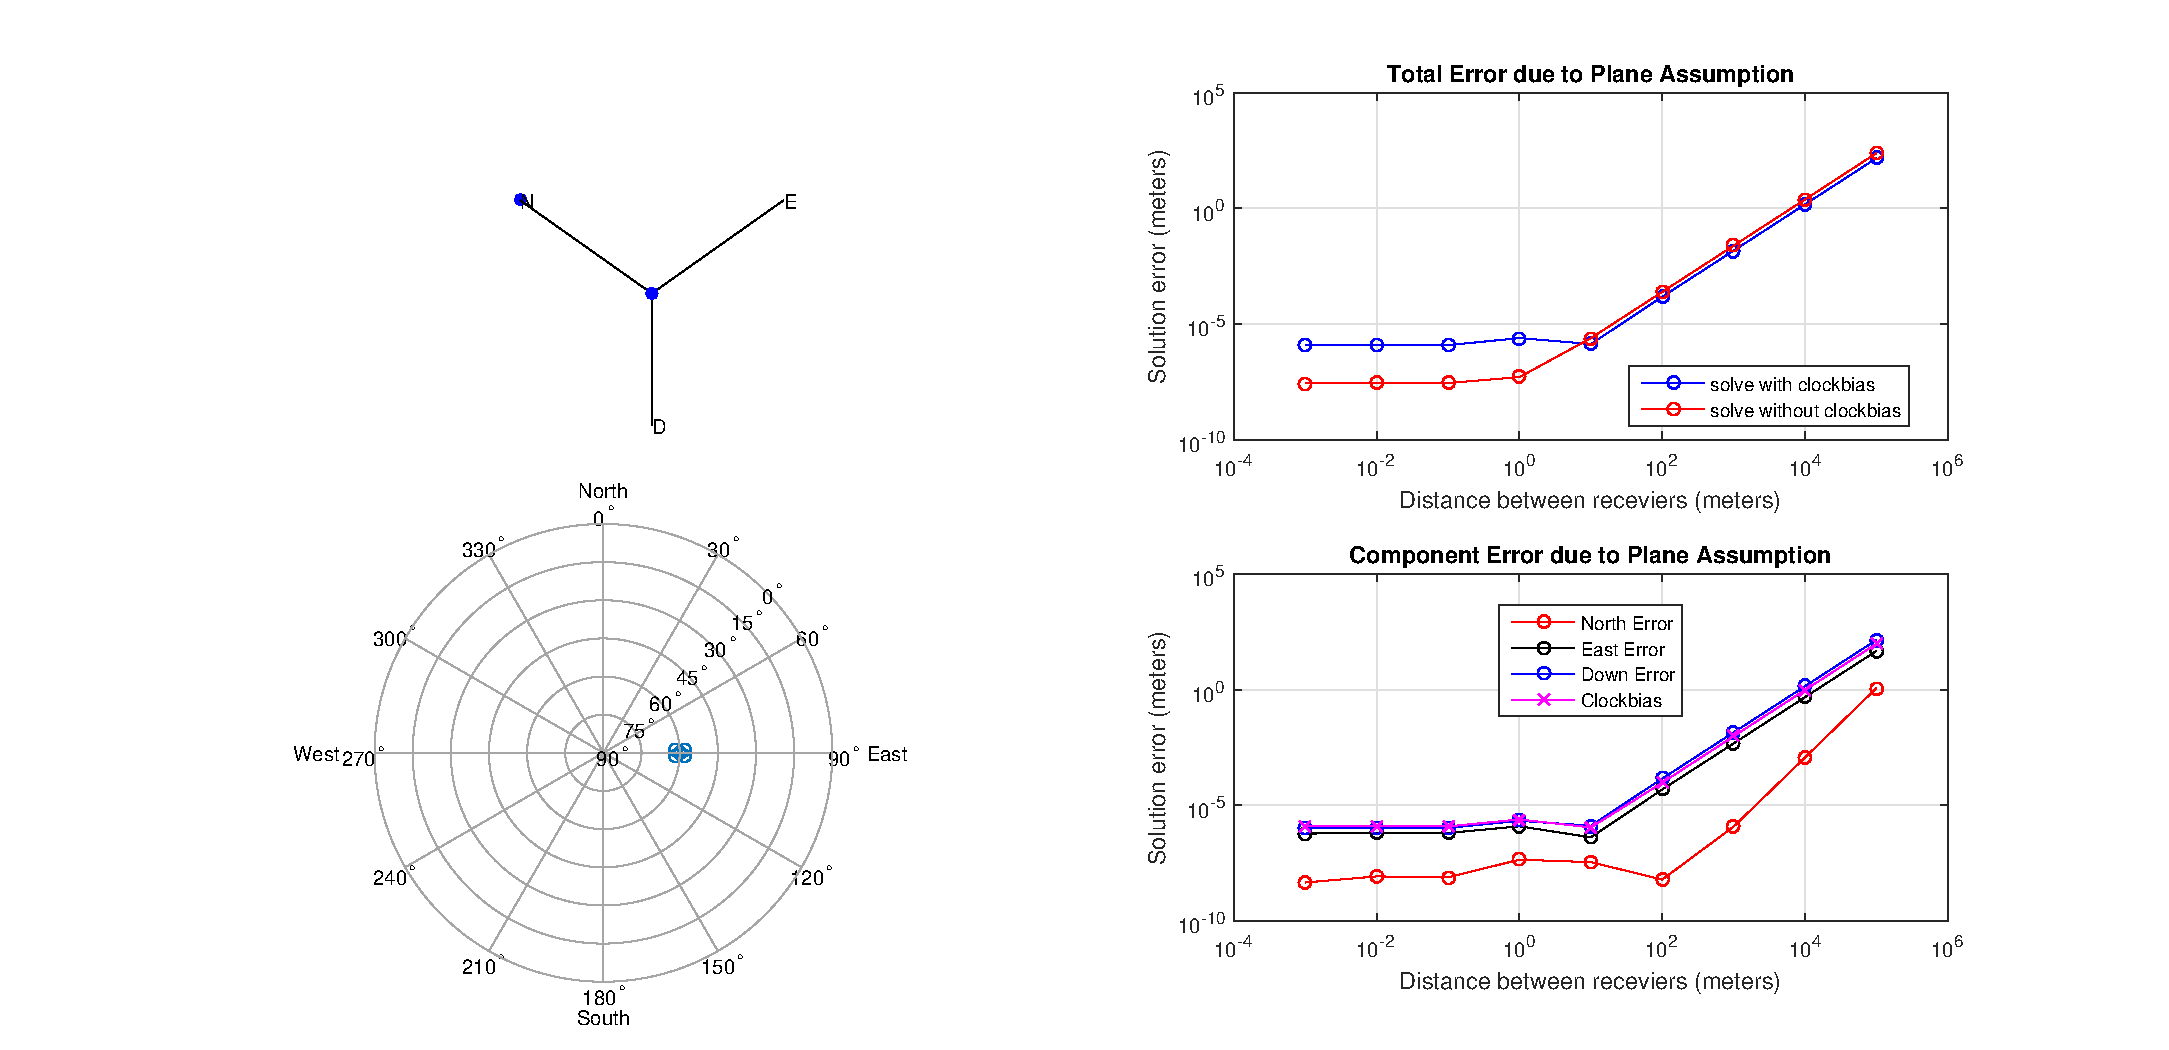
\includegraphics[trim = 3cm 0 0 0,clip,width=\linewidth]{ChapterExperiments/Figures/plane_ALLE_north_9060}
\end{figure}



The configuration of the satellites were also varied. 

NOTE: When the satellites are in a cluster, the planes are very close together with minimal difference between them.
with no errors in the system, the clockbias still went nuts with the constrain (tr-t1) on D
the values of x,y,z are so big for the large differences that a small clockbias is proportionally the minimum
SHOW WITH AND WITHOUT SOLVING FOR CLOCKBIAS
- the excessive clock bias is trying to minimise the error due to the plane assumption



\begin{figure}
\centering
\caption{}
\label{fig:plane_ALLE_north_0075}
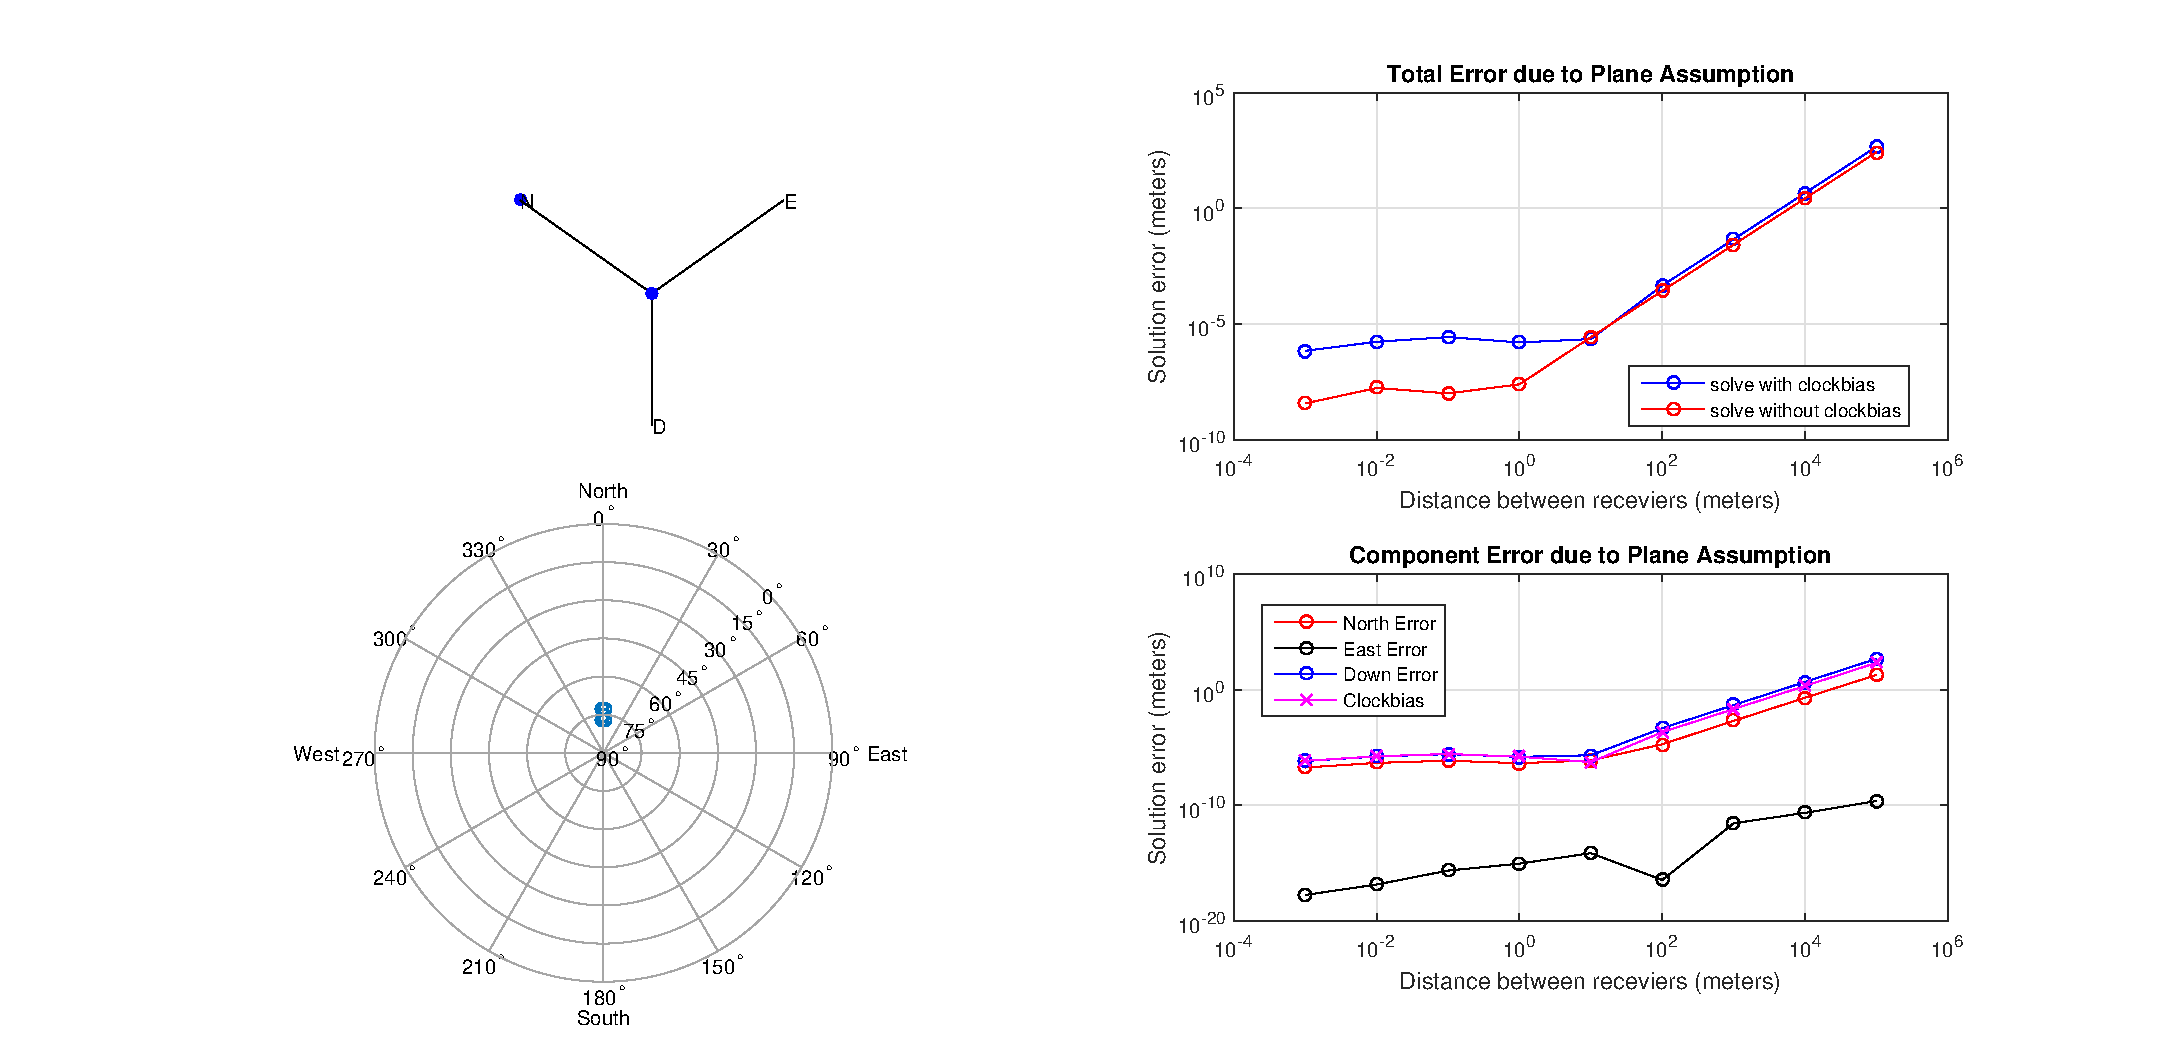
\includegraphics[width=0.7\linewidth]{ChapterExperiments/Figures/plane_ALLE_north_0075}
\end{figure}

%% using main_fn_planesats
\begin{figure}
\centering
\caption{North}
\label{fig:plane_total_north1_pow4}
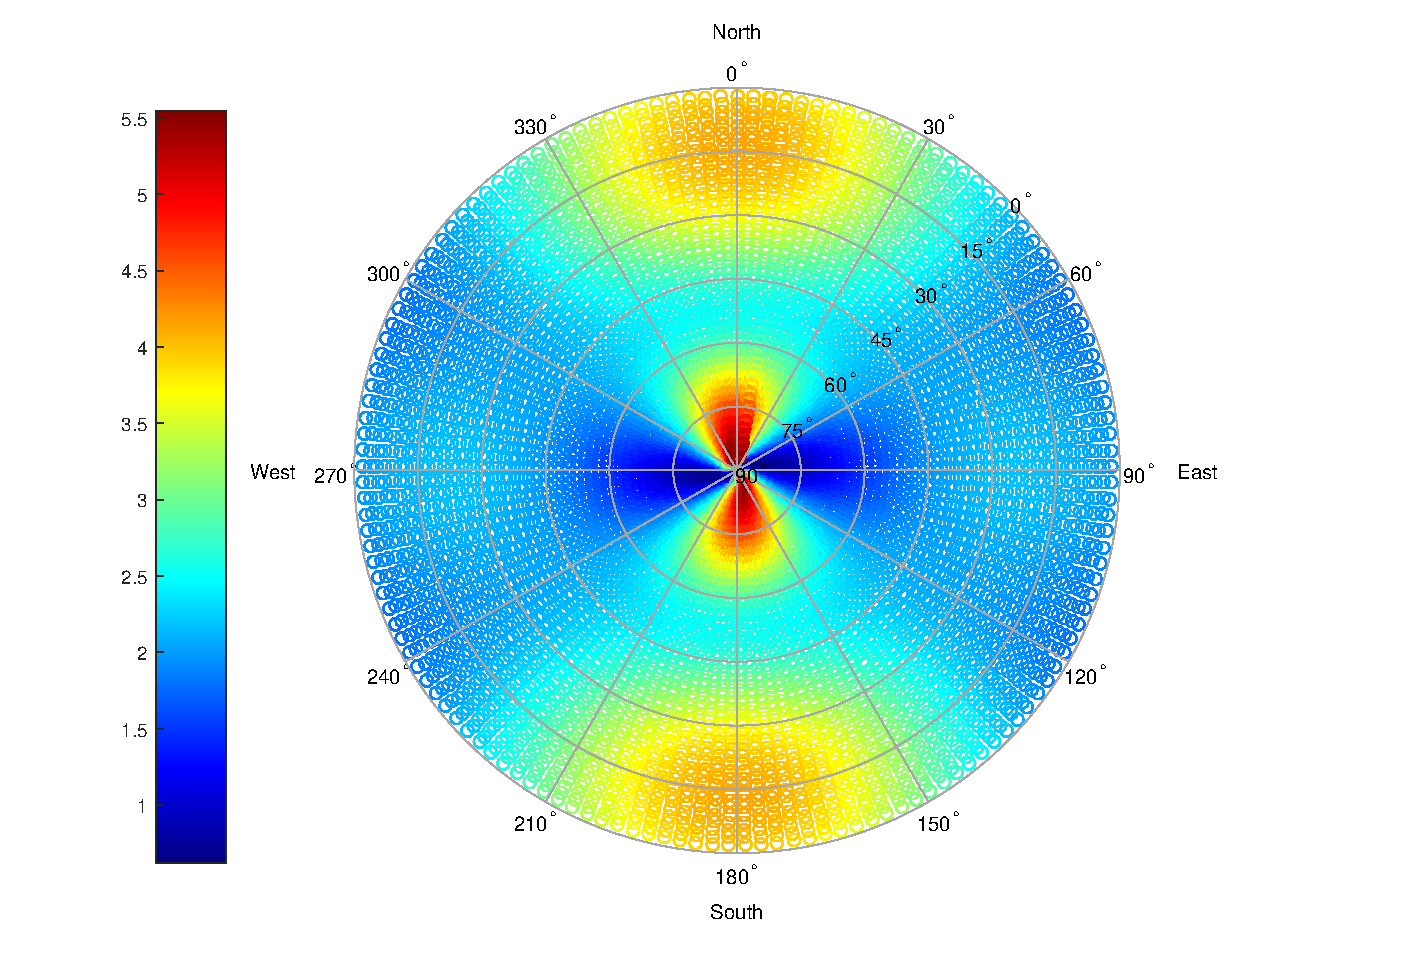
\includegraphics[width=0.7\linewidth]{ChapterExperiments/Figures/plane_total_north1_pow4}
\end{figure}

\begin{figure}
\centering
\caption{East}
\label{fig:plane_total_east_pow4}
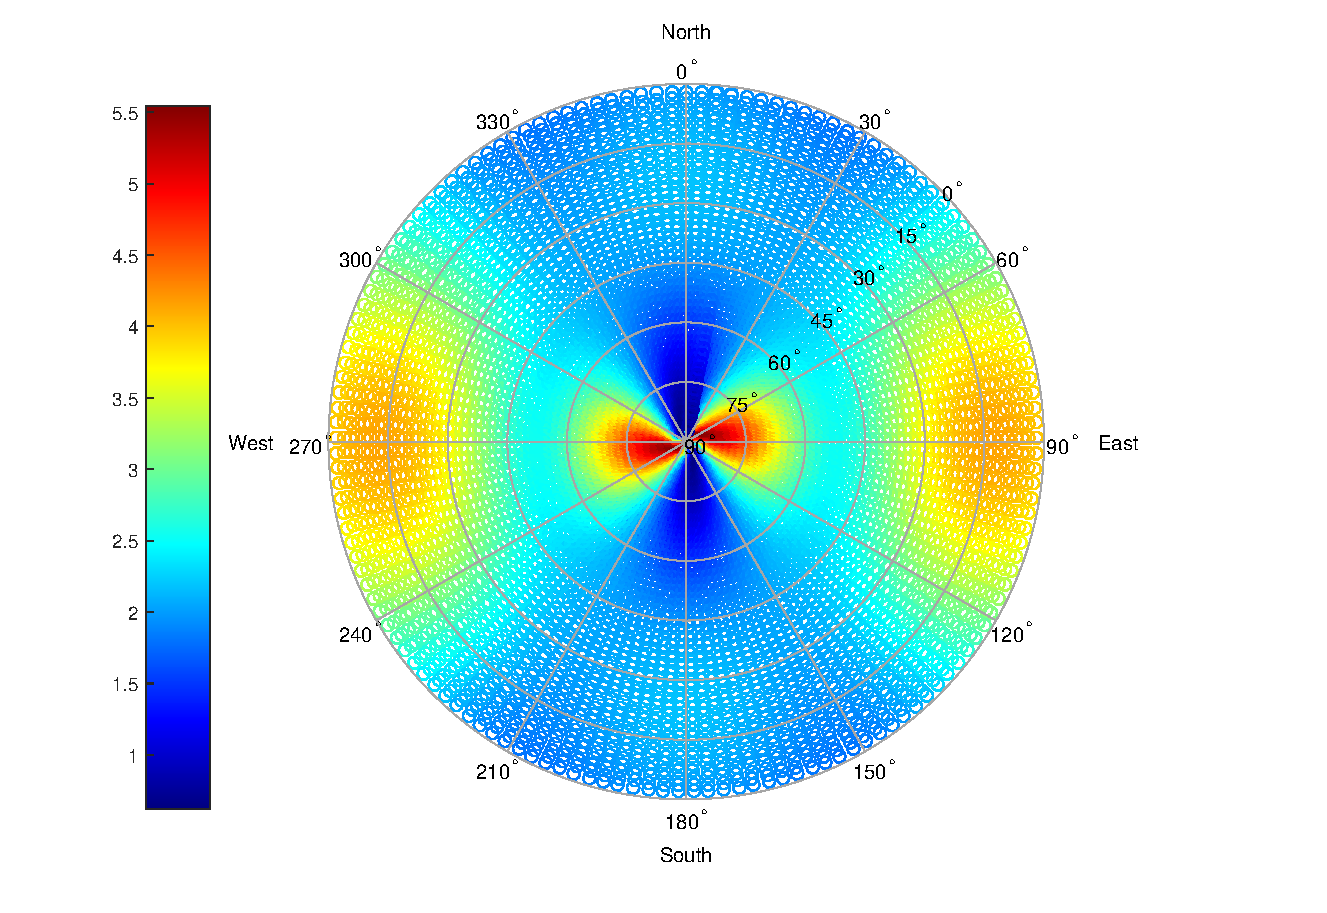
\includegraphics[width=0.7\linewidth]{ChapterExperiments/Figures/plane_total_east_pow4}
\end{figure}

\begin{figure}
\centering
\caption{Down}
\label{fig:plane_total_down_pow4}
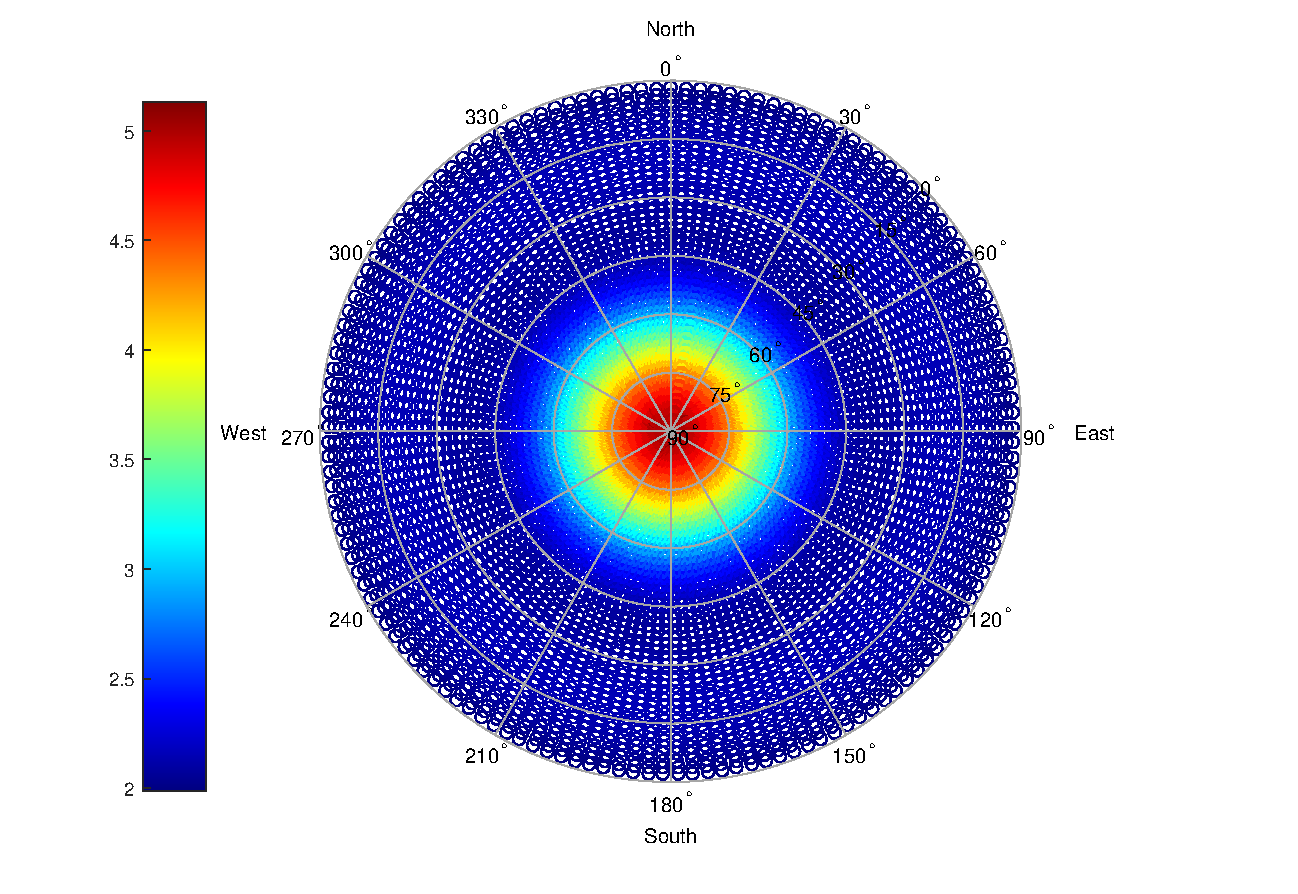
\includegraphics[width=0.7\linewidth]{ChapterExperiments/Figures/plane_total_down_pow4}
\end{figure}

\begin{figure}
\centering
\begin{subfigure}{0.49\textwidth}
\centering
\caption{Config:North, Error:North}
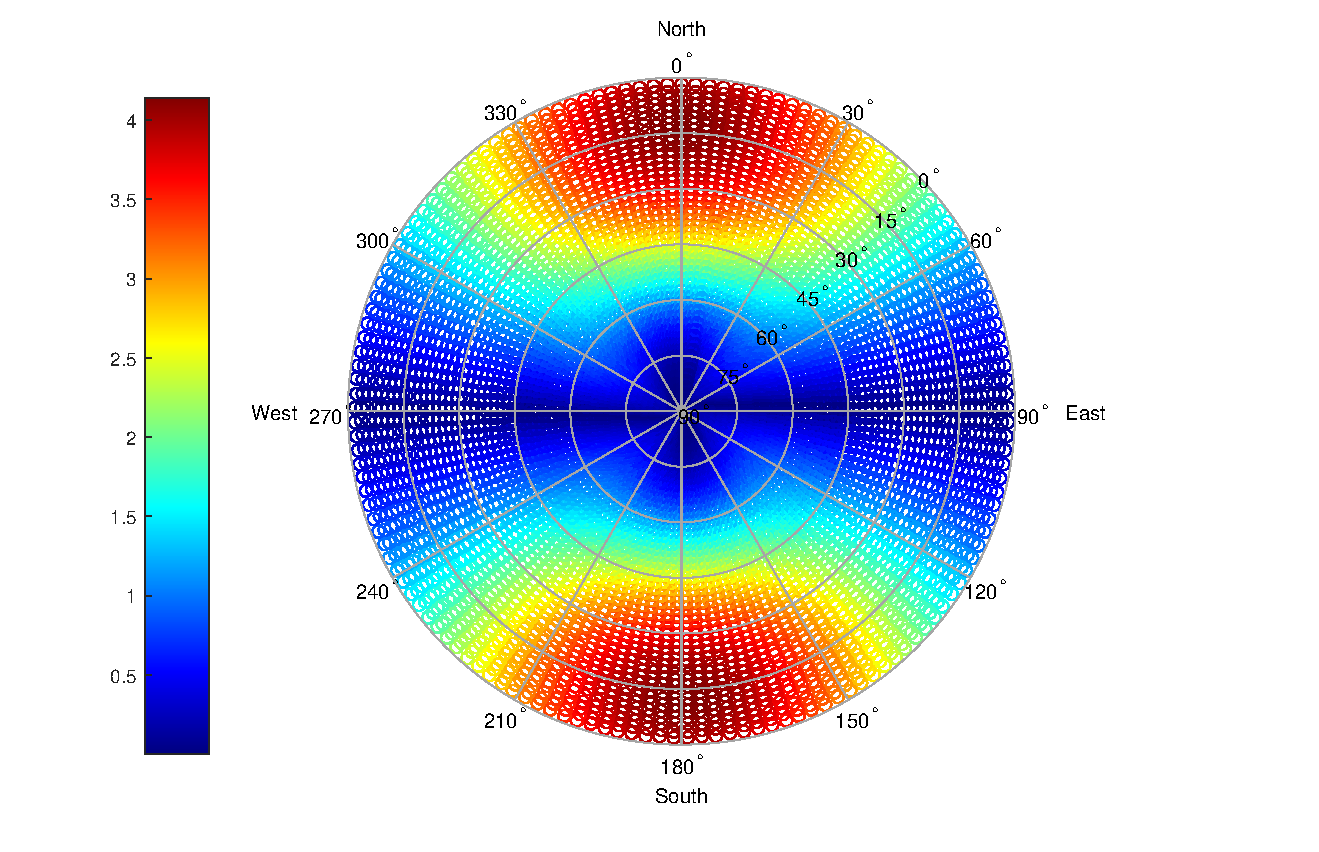
\includegraphics[width =\linewidth]{ChapterExperiments/Figures/plane_Enorth_north_pow4}
\end{subfigure}
\begin{subfigure}{0.49\linewidth}
\centering
\caption{Config:Down, Error:North}
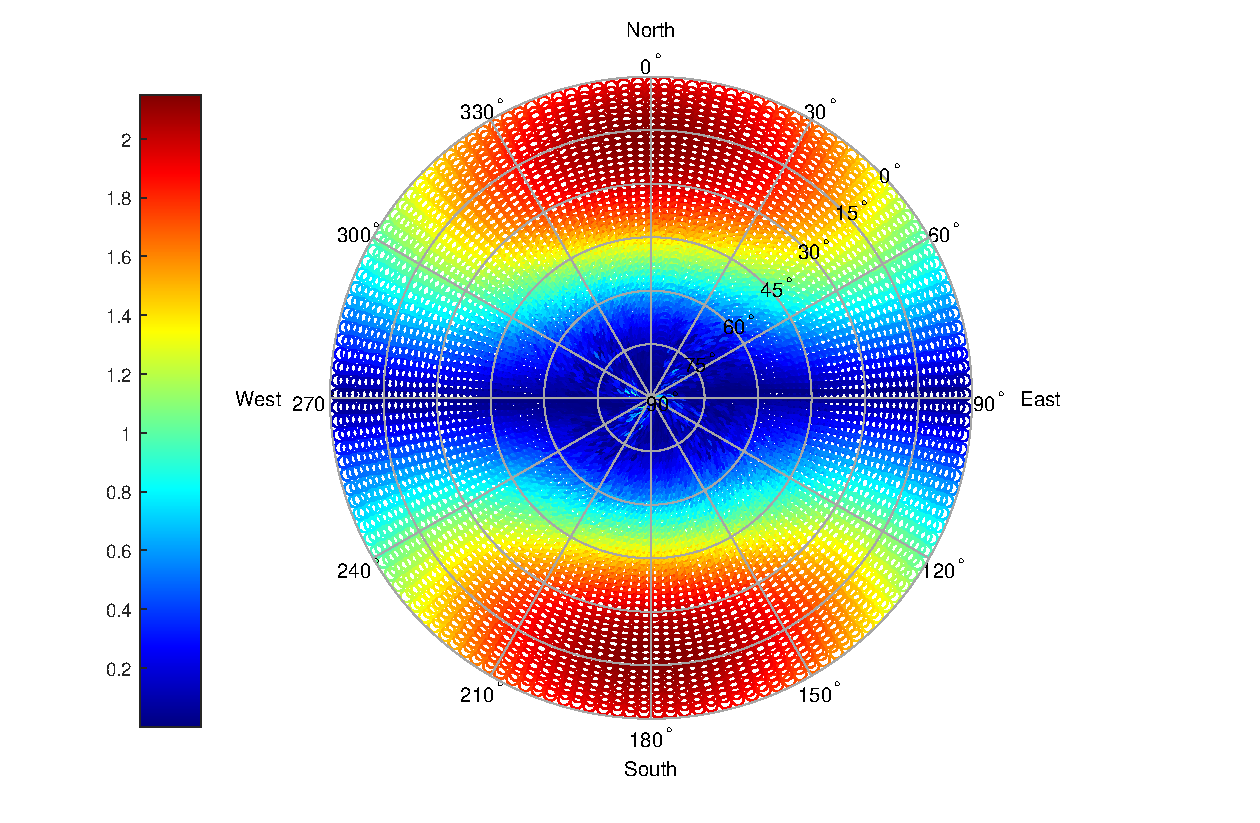
\includegraphics[width = \linewidth]{ChapterExperiments/Figures/plane_Enorth_down_pow4}
\end{subfigure}
\begin{subfigure}{0.49\textwidth}
\centering
\caption{Config:North, Error:East}
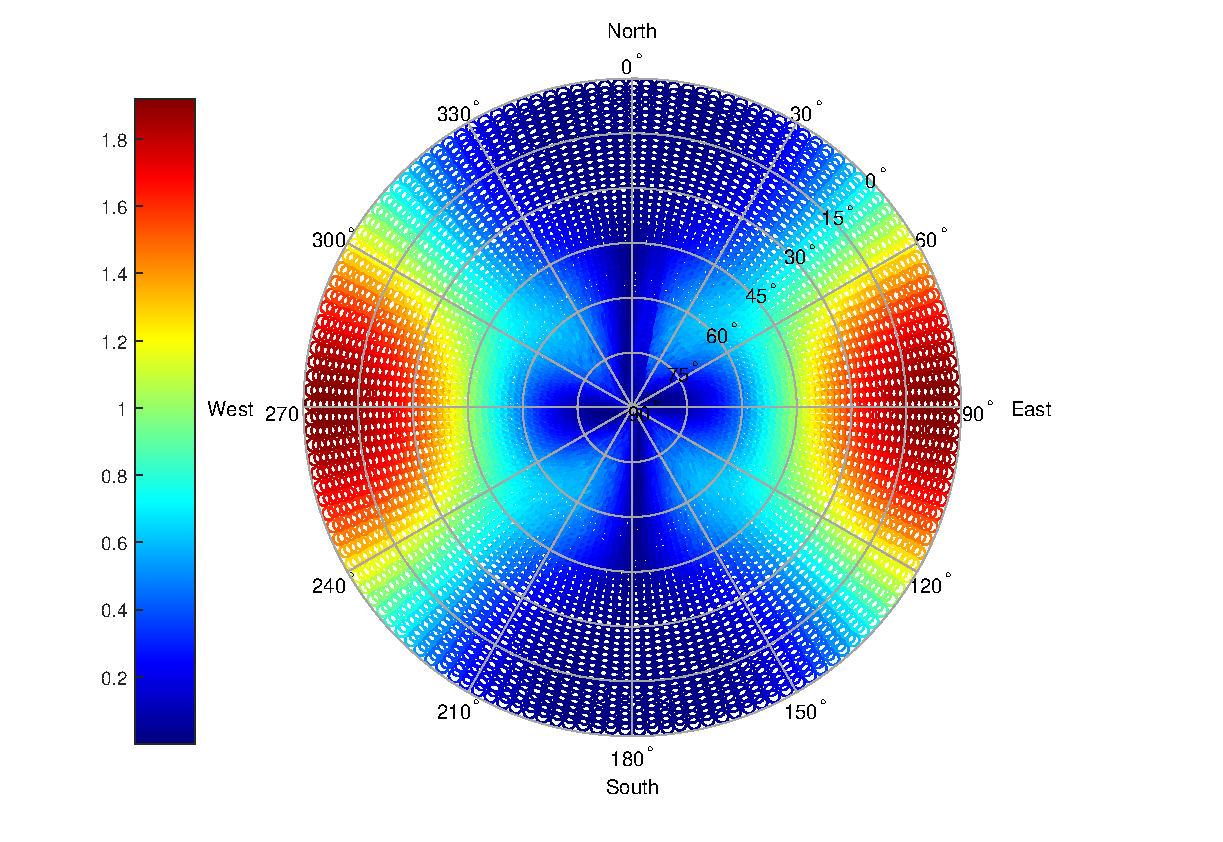
\includegraphics[width =\linewidth]{ChapterExperiments/Figures/plane_Eeast_north_pow4}
\end{subfigure}
\begin{subfigure}{0.49\linewidth}
\centering
\caption{Config:Down, Error:East}
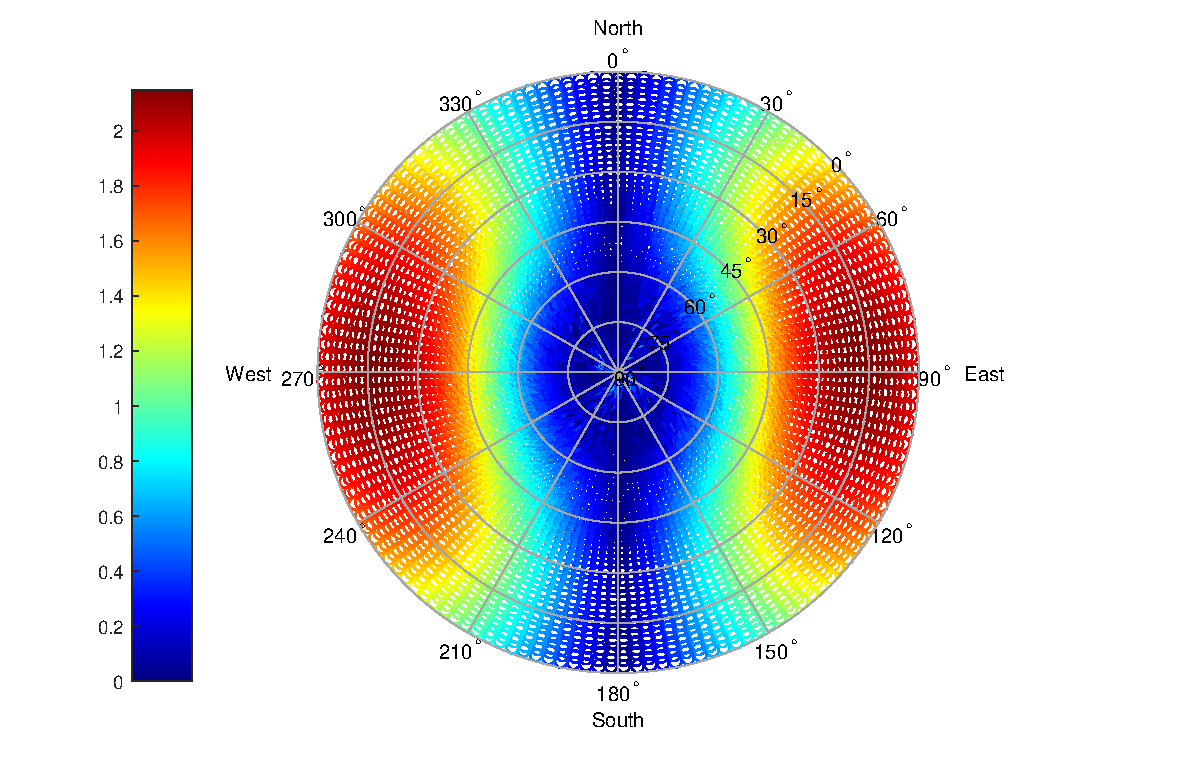
\includegraphics[width = \linewidth]{ChapterExperiments/Figures/plane_Eeast_down_pow4}
\end{subfigure}
\begin{subfigure}{0.49\textwidth}
\centering
\caption{Config:North, Error:Down}
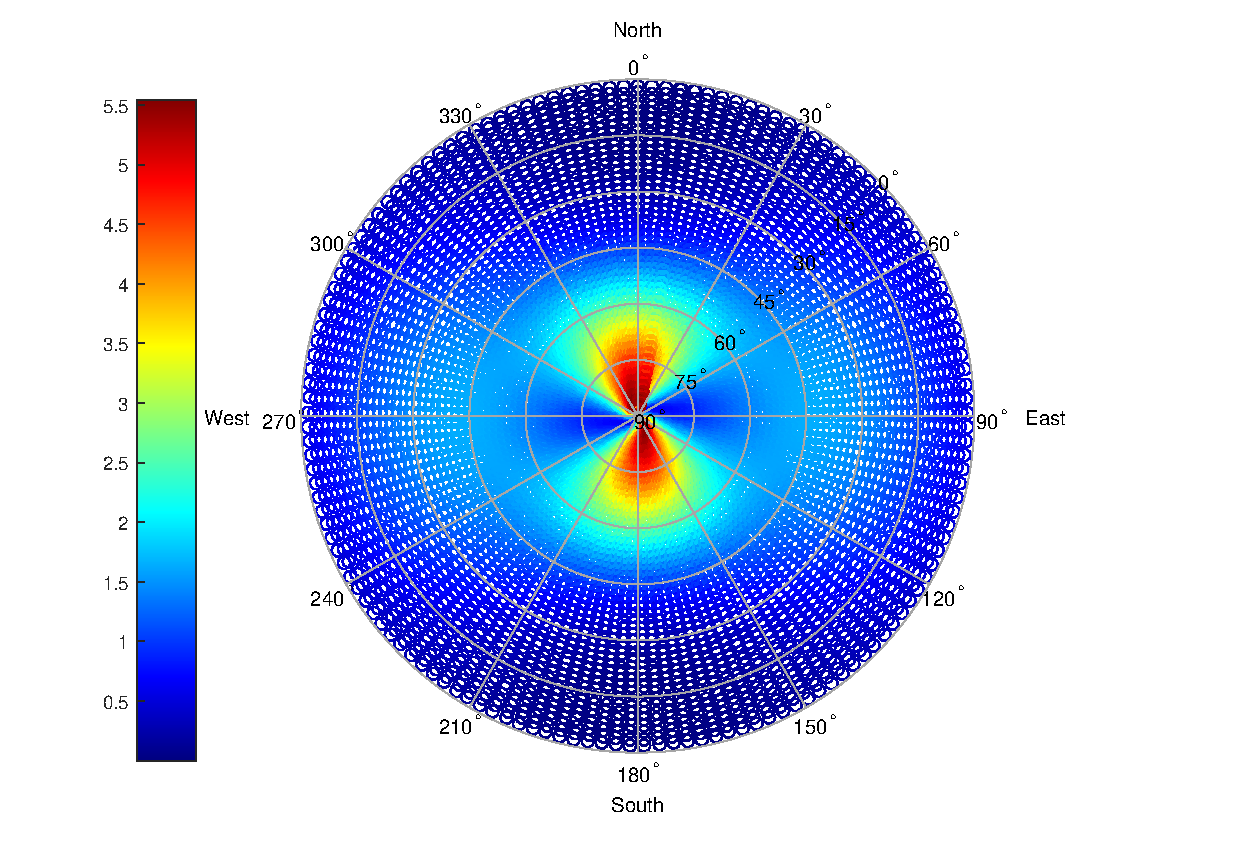
\includegraphics[width =\linewidth]{ChapterExperiments/Figures/plane_Edown_north_pow4}
\end{subfigure}
\begin{subfigure}{0.49\linewidth}
\centering
\caption{Config:Down, Error:Down}
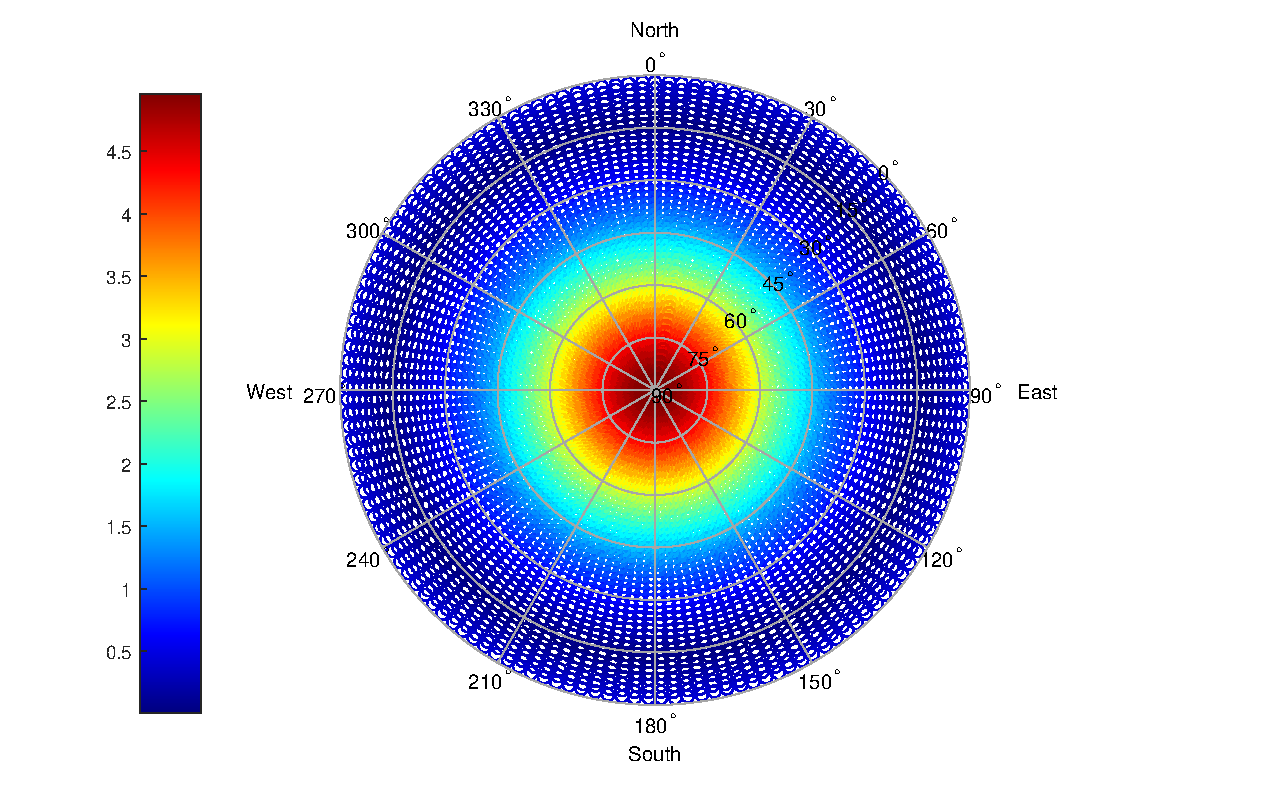
\includegraphics[width = \linewidth]{ChapterExperiments/Figures/plane_Edown_down_pow4}
\end{subfigure}
\end{figure}
